\chapter{Compensador Analogico} \chapterlabel{Informe/6-CompensadorAnalogico} \label{cap:Compensador Analogico}

\section{Lazo de realimentación Interno}
\subsection{Diseño de la red de adelanto de fas}
\noindent Se plantea una compensación como la que se muestra en la figura \ref{fig:diag-en-bloques-comp}. Está compuesta por un lazo de control interno con un controlador por adelanto de fase para lograr estabilizar el sistema, y un lazo de control externo con un integrador para eliminar el error en régimen permanente.

\begin{figure}[H]
	\centering
	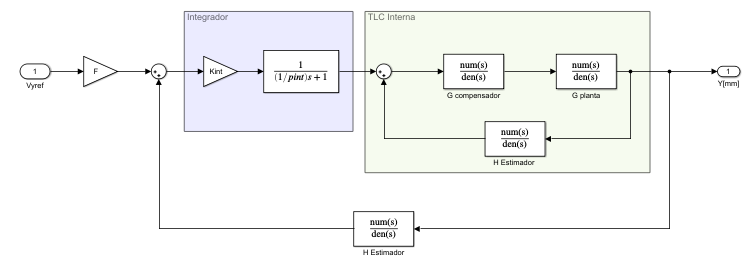
\includegraphics[scale=0.8]{Diagrama-en-bloques-comp.png}
	\caption{Diagrama del sistema completo.}
	\label{fig:diag-en-bloques-comp}
\end{figure}

\subsubsection{Análisis de estabilidad con masa de 30Kg}

\noindent Para el análisis del compensador analógico se parte de las transferencias de la planta $G_{p}(s)$ para una masa de 30 Kg, del controlador de corriente $G_{iL}(s)$  y del lazo de realimentación $H_{estim}$. A partir de ellas se obtiene  la transferencia a lazo abierto total $GH_T(s)$ mostrado en la ecuación \ref{eq_GT2}.


\begin{equation*} \label{eq_GT1}
	GH_T(s)=G_{p}(s)*G_{iL}(s)*H_{estim} 
\end{equation*}

\begin{equation} \label{eq_GT2}
		GH_T(s)=\frac{0.38}{(1-(\frac{s}{70}))(\frac{S}{12.17\ }+1)(1+\frac{s}{1\ Krad/s}){(1+\frac{s}{60\ Krad/s})}^2 }	
\end{equation}

\noindent A continuación se procede a analizar la respuesta en frecuencia de $GH_T$ y a diseñar un compensador adecuado. Luego, se verificará la estabilidad para una masa de 1 Kg, que corresponde a la mínima con la que trabaja el sistema.


\noindent Con la transferencia de la ecuación  \ref{eq_GT2} se  grafica el diagrama de Bode y el diagrama de Nyquist. Estos se muestran en las figuras \ref{fig:Diag_Bode_lazo_abierto_30kg} y \ref{fig:Diag_Nyquist_lazo_abierto_30kg} respectivamente.

\begin{figure}[H]
	\centering
	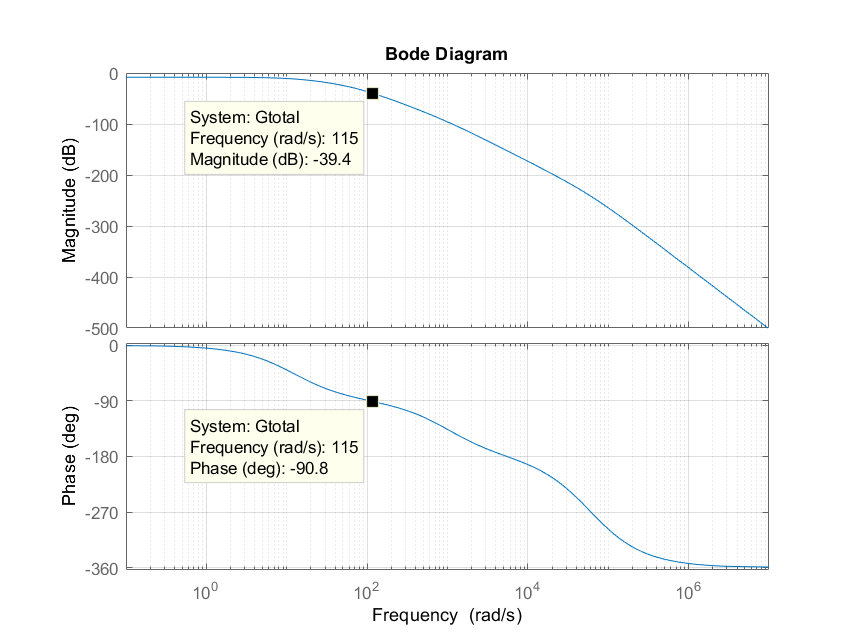
\includegraphics[scale=0.6]{bode_planta_30kg.png}
	\caption{Diagrama de Bode de lazo abierto $GH_T$ con M=30 Kg.}
	\label{fig:Diag_Bode_lazo_abierto_30kg}
\end{figure}

\begin{figure}[H]
	\centering
	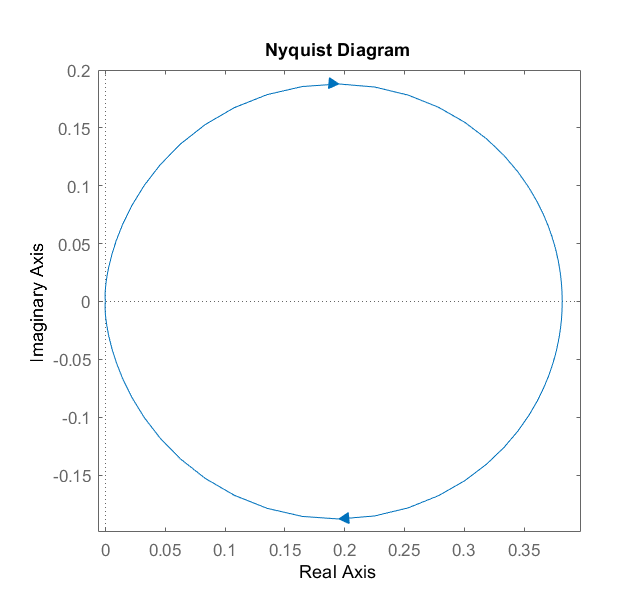
\includegraphics[scale=0.6]{nyquist_planta_30kg.png}
	\caption{Diagrama de Nyquist de GHT con M=30 Kg.}
	\label{fig:Diag_Nyquist_lazo_abierto_30kg}
\end{figure}

\noindent Para poder observar mejor la forma del Nyquist se hace un acercamiento en torno al origen como se muestra en la figura \ref{fig:Diag_Nyquist_lazo_abierto_zoom_30kg}.

\begin{figure}[H]
	\centering
	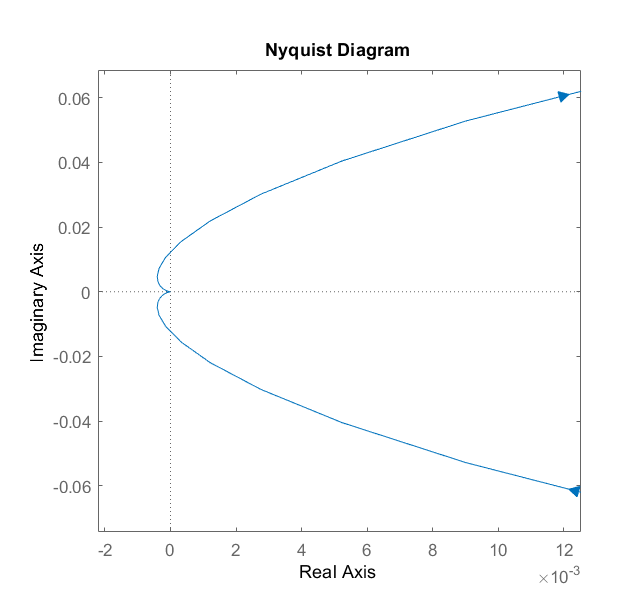
\includegraphics[scale=0.6]{nyquist_planta_zoom_30kg.png}
	\caption{Zoom del diagrama de Nyquist de GHT con M=30 Kg.}
	\label{fig:Diag_Nyquist_lazo_abierto_zoom_30kg}
\end{figure}

En la figura \ref{fig:rlocus_m30kg} se puede observar el lugar de raíces de $GH_{T}$ y en la \ref{fig:rlocus_m30kg_zoom} se muestra un acercamiento.

\begin{figure}[H]
	\centering
	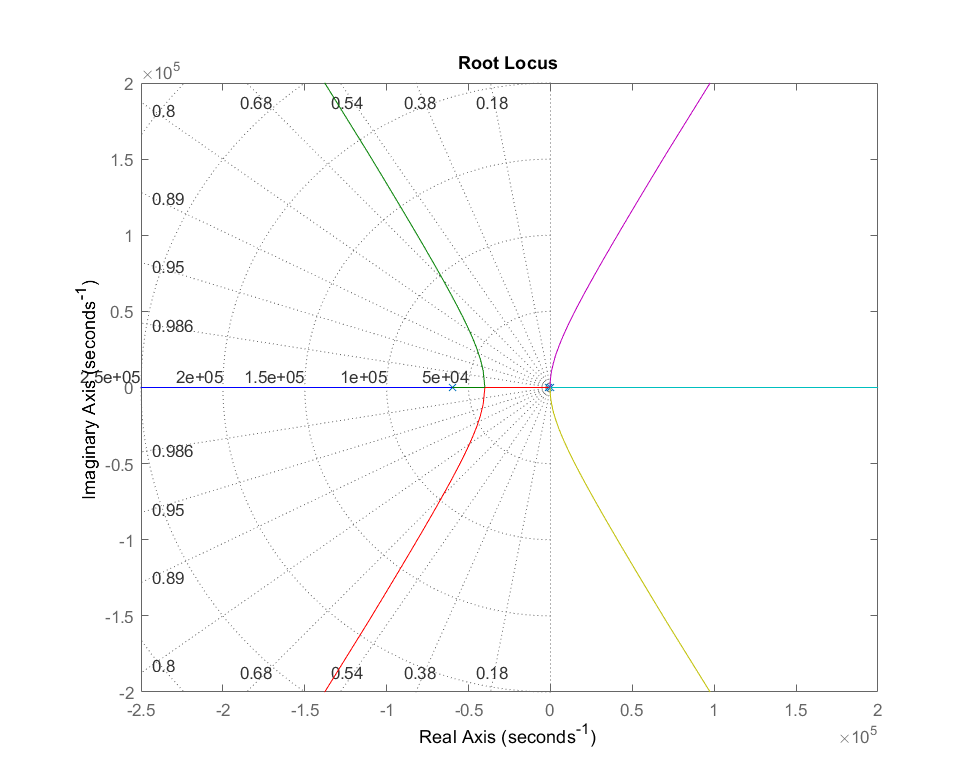
\includegraphics[scale=0.6]{rlocus_planta_30kg.png}
	\caption{Lugar de raíces de $GH_{T}$ con M=30Kg.}
	\label{fig:rlocus_m30kg}
\end{figure}

\begin{figure}[H]
	\centering
	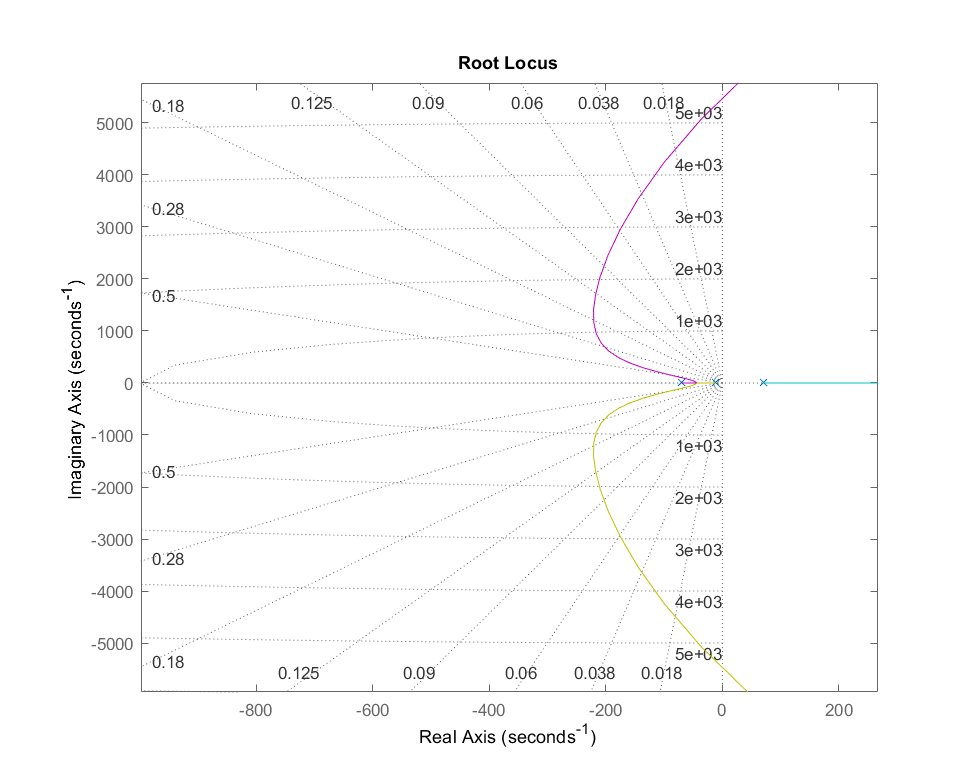
\includegraphics[scale=0.6]{rlocus_planta_30kg_zoom.png}
	\caption{Zoom del lugar de raíces de GHT con M=30Kg.}
	\label{fig:rlocus_m30kg_zoom}
\end{figure}

\noindent Como se observa en la figura \ref{fig:rlocus_m30kg_zoom}, $GH_{T}$ tiene un polo en el semiplano derecho. Por lo tanto, a partir del Nyquist se puede determinar:

\noindent Zona 1: Z=N+P=0+1=1 $\mathrm{\to}$ Inestable 

\noindent Zona 2: Z=N+P=1+1=2 $\mathrm{\to}$ Inestable

\noindent De esta forma, no es posible que el sistema sea estable. Para lograrlo se realimentar\'{a} positivamente y se generar\'{a} una zona en el diagrama de Nyquist donde N=-1. Para ello es necesario aumentar la fase para que pueda superar el valor de 0$\mathrm{{}^\circ}$.  Para que esto se cumpla, el diagrama de Nyquist deber\'{i}a tener una forma como la  mostrada en la figura \ref{fig:nyquist-deseado-analog}.

\begin{figure}[H]
	\centering
	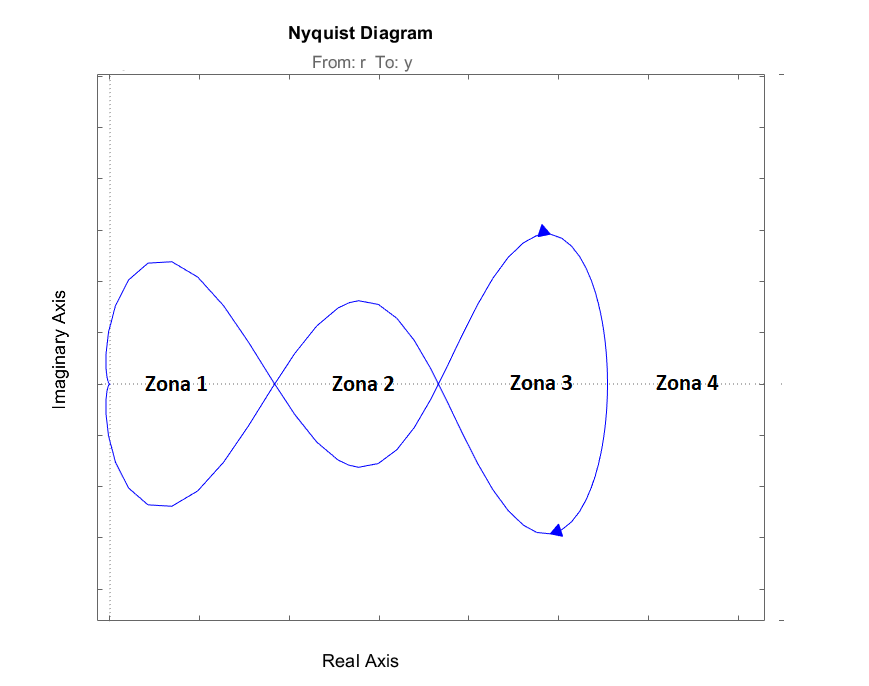
\includegraphics[scale=0.7]{Nyquist-deseado-analog.png}
	\caption{Forma del diagrama de Nyquist deseado.}
	\label{fig:nyquist-deseado-analog}
\end{figure}

\noindent Para poder lograr el aumento de fase mencionado se utiliza una red de adelanto de fase. Se debe tener en cuenta que el m\'{o}dulo de la transferencia de lazo abierto en el primer cruce de la fase por 0$\mathrm{{}^\circ}$ debe ser mayor a 0 dB y, en el segundo cruce, menor. De esta forma, al observar la figura \ref{fig:Diag_Bode_lazo_abierto_30kg} se decide adelantar la fase 100º en aproximadamente 200 rad/s. Esto se logra usando dos redes de adelanto de fase de 65$\mathrm{{}^\circ}$ cada una.

\noindent Ecuaciones de dise\~{n}o:

\begin{equation*}
	\begin{aligned}
		W_0 &=200\ r/s\\
		{\varphi }_{max} &=65\textrm{º}\\
		\alpha &=\frac{1+sen{\varphi }_{max}}{1-sen{\varphi }_{max}}=20.346491\\
		W_c &=\frac{W_0}{\sqrt{\alpha }}=\ 44.3\ r/s\\
		W_p &=\sqrt{\alpha }*W_0=902.1\ r/s\\
	\end{aligned}
\end{equation*} 
\noindent Finalmente se llega a la transferencia del controlador:

\begin{equation}  
	G_c(s)=K*{[20.346*\frac{(s+44.3)}{(s+902.1)}]}^2
\end{equation} 

\noindent En la figura \ref{fig:bode-analog-compensado-para-k-1} se muestra el diagrama de bode de ${GH}_T*G_C$ con $K=1$. Se puede observar que la ganancia $K$ puede adoptar valores desde 15 dB hasta 35 dB. Considerando que el sistema debe soportar una masa variable entre 1 kg y 30 kg, y que la ganancia de la transferencia de la planta para 1 kg es de 5.5 veces (14 dB) mayor que para 30 kg, se puede adoptar una ganancia del compensador que mantenga la estabilidad para estos dos casos. Es decir, la ganancia m\'{i}nima es de 15 dB y la m\'{a}xima es de 35 dB - 14 dB = 21 dB. Por lo tanto, se elige que el cruce por cero de la ganancia se encuentre ahora en 88 rad/s, lo que significa que $K=20dB\ \equiv \ 10\ veces$.


\begin{figure}[H]
	\centering
	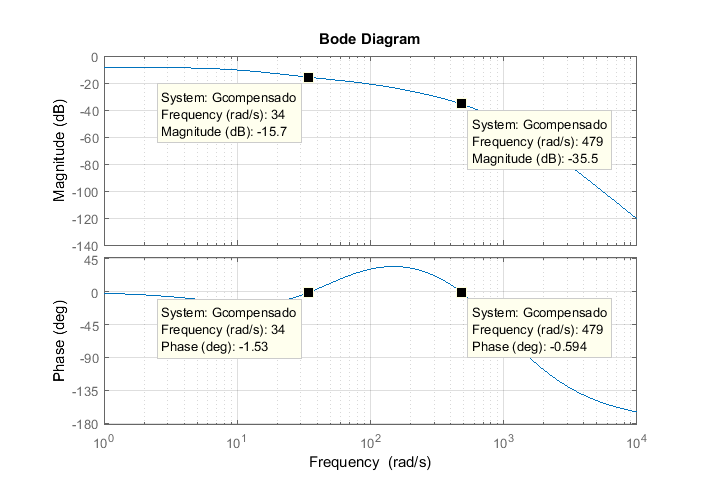
\includegraphics[scale=0.85]{Bode-k-1-M-30.png}
	\caption{Diagrama de Bode de $GH_T*G_C$ para K=1 y M=30 kg.}
	\label{fig:bode-analog-compensado-para-k-1}
\end{figure}

\noindent En la figura \ref{fig:bode-analog-compensado-para-k-10} se muestra el diagrama de Bode considerando la ganancia del compensador. En ella se puede observar que se  cumple con el criterio de estabilidad, puesto que en el primer cruce por 0º, la magnitud es mayor a 0 dB y en el segundo cruce, menor. Adem\'{a}s, en la figura \ref{fig:nyquist-analog-para-k-10} se puede ver que la forma del diagrama de Nyquist es como la deseada.

\begin{figure}[H]
	\centering
	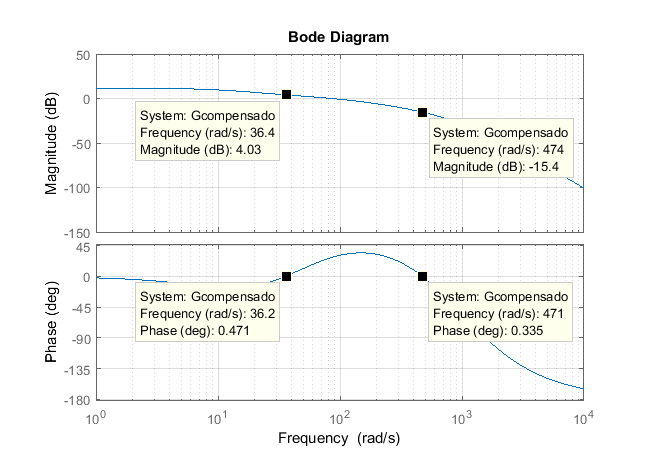
\includegraphics[scale=0.85]{Bode-k-10-M-30.png}
	\caption{Diagrama de Bode de $GH_{T}*GC$ para K=10 y M=30 Kg.}
	\label{fig:bode-analog-compensado-para-k-10}
\end{figure}

\begin{figure}[H]
	\centering
	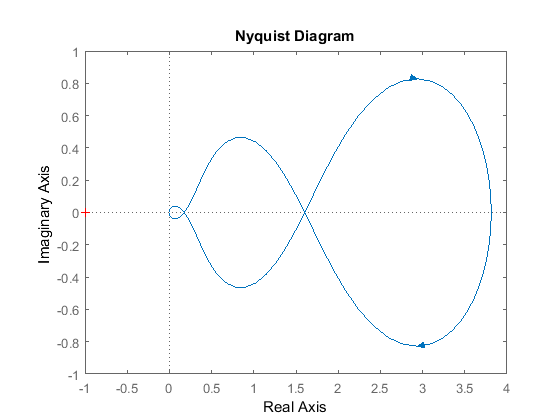
\includegraphics[scale=0.85]{Nyquist-k-10-M-30.png}
	\caption{Diagrama de Nyquist de GHT*GC para K=10 y M=30 Kg.}
	\label{fig:nyquist-analog-para-k-10}
\end{figure}

\noindent En la figura \ref{fig:rta-escalon-k-10-m-30} se puede observar la respuesta al escalón del sistema con masa de 30 Kg.

\begin{figure}[H]
	\centering
	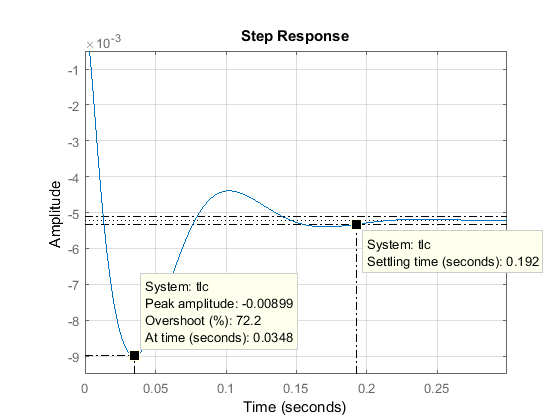
\includegraphics[scale=0.85]{Respuesta-al-escalon-K-10-M-30Kg.png}
	\caption{Respuesta al escalón para M=30 Kg.}
	\label{fig:rta-escalon-k-10-m-30}
\end{figure}

\subsubsection{Análisis de estabilidad con masa de 1 Kg}

\noindent En esta secci\'{o}n se verifica la estabilidad del sistema  para el caso en que la masa sea de 1 Kg, utilizando el compensador dise\~{n}ado para el caso de masa m\'{a}xima. Para ello, se analizan los diagramas de Bode y Nyquist mostrados en las figuras \ref{fig:bode-analog-para-M-1Kg} y \ref{fig:nyquist-analog-para-M-1Kg}. Adem\'{a}s, en la figura \ref{fig:respuesta-analog-al-escalon-para-M-1Kg} puede observarse la respuesta al escal\'{o}n. A partir de ellos, es posible verificar que efectivamente el sistema resulta estable para todo el rango de masas en el que opera el sistema. 


\begin{figure}[H]
	\centering
	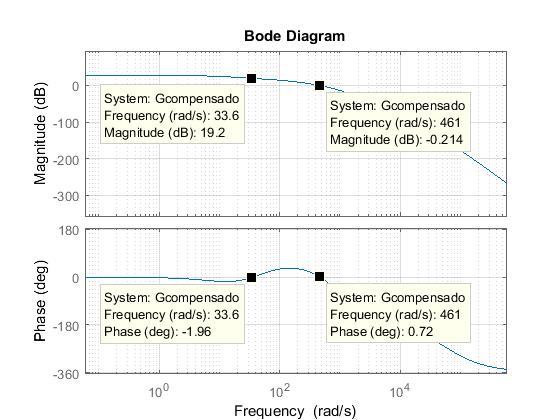
\includegraphics[scale=1]{bodecompensado1kg.png}
	\caption{Diagrama de Bode de $GH_T*G_C$ para M=1 Kg.}
	\label{fig:bode-analog-para-M-1Kg}
\end{figure}

\begin{figure}[H]
	\centering
	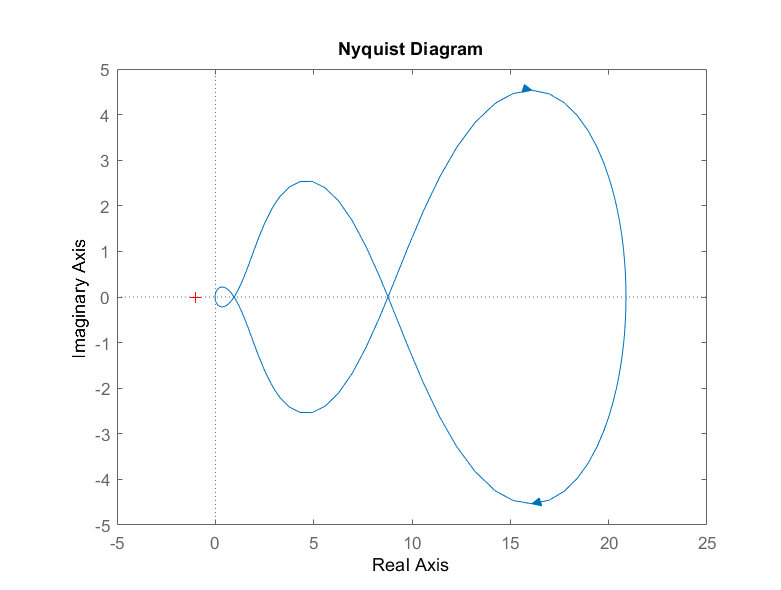
\includegraphics[scale=0.7]{nyquistcompensado1kg.png}
	\caption{Diagrama de Nyquist de $GH_T*GC$ para M=1 Kg.}
	\label{fig:nyquist-analog-para-M-1Kg}
\end{figure}

\begin{figure}[H]
	\centering
	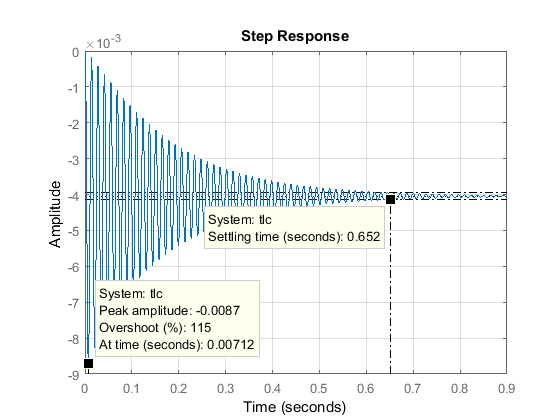
\includegraphics[scale=1]{rtaescaloncompensado1kg.png}
	\caption{Respuesta al escalón para M=1 Kg.}
	\label{fig:respuesta-analog-al-escalon-para-M-1Kg}
\end{figure}

\subsubsection{Implementación circuital de la red de adelanto de fase}

\begin{figure}[H]
	\centering
	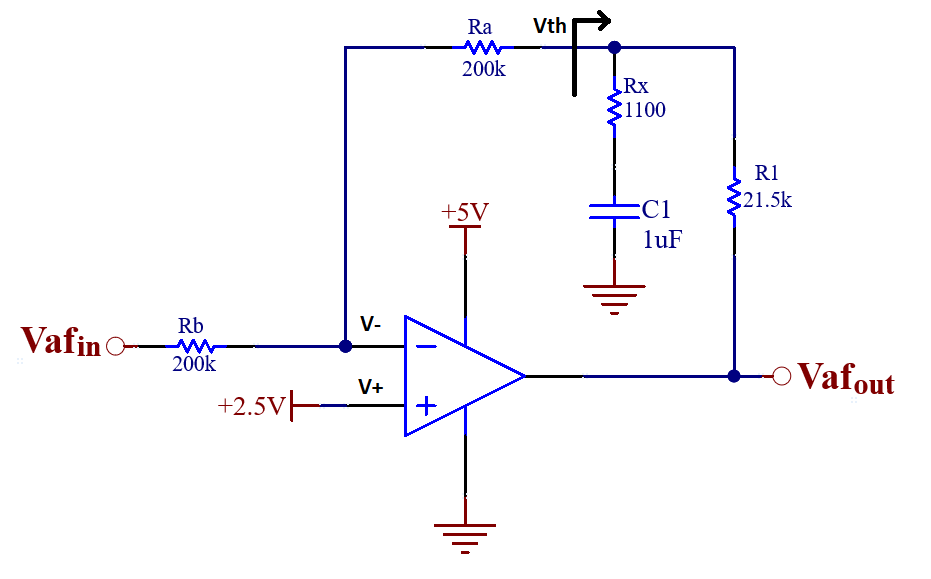
\includegraphics[scale=0.6]{Red-adelanto-fase.png}
	\caption{Diseño circuital de una red de adelanto de fase.}
	\label{fig:red-adelanto-fase}
\end{figure}


\noindent Para cada etapa del compensador por adelanto, se utilizará la topología mostrada en la figura \ref{fig:red-adelanto-fase}. Consiste en  un polo y cero con ganancia unitaria (si Ra = Rb). Luego se agrega la ganancia como una etapa separada.

\noindent La transferencia de lazo cerrado de esta etapa es:

\begin{equation} 
	\frac{V_{out}}{V_{in}}= - \frac{R_a}{R_b}*\frac{1+sC(R_x+R1)}{1+sCR_x}
\end{equation}

\noindent Por lo tanto, para tener polo = 902.1 Hz y zero = 44.3, y eligiendo el capacitor C = 1uF, resulta $R_x$ = 1100 y R1 = 21.5K. Además, se elige $R_a$ = $R_b$ = 200k para ganancia unitaria. Luego, la ganancia del compensador se obtiene con una etapa amplificadora.
Para ello, se utiliza un amplificador operacional como se muestra en la figura \ref{fig:ganancia-compensador}. Para lograr una ganancia de K=10 se utiliza $R_{322}$ = 1K y $R_{323}$ = 10K.


\begin{figure}[H]
	\centering
	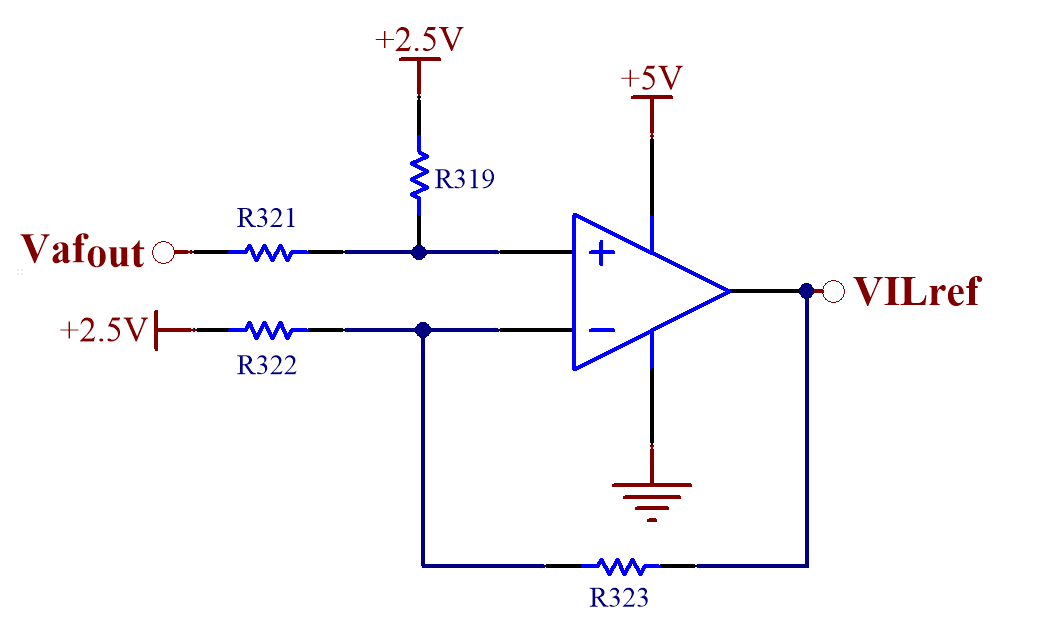
\includegraphics[scale=0.6]{Ganancia-compensador.png}
	\caption{Etapa de ganancia del compensador.}
	\label{fig:ganancia-compensador}
\end{figure}

\section{Lazo de realimentación externo}
\subsection{Diseño de Integrador}

\noindent Se plantea un lazo de realimentaci\'{o}n externo como se muestra en la  figura \ref{fig:diag-en-bloques-comp}.

\noindent En el lazo de realimentaci\'{o}n interno act\'{u}a el compensador por adelanto de fase dise\~{n}ado previamente y, en el externo, un controlador del tipo integral. De esta forma, se logra suavizar la respuesta al escal\'{o}n del sistema y eliminar el error en r\'{e}gimen permanente.


\noindent Para el an\'{a}lisis se considera como realimentaci\'{o}n: 

\[H_{estim}=\frac{V_{estim}}{Y[m]}= - \frac{259.6}{(1 + \frac{s}{1Kr/s})*(1+\frac{s}{60Kr/s})^2}\] 

\noindent La cadena de avance con masa de 30 Kg es:

\[G[m=30]=Tlc_{interna}(s)[m=30]*G_{Integrador}\] 

\noindent Se  plantea un compensador del tipo :

\[Ginteg\ =\ kint\ *\ \frac{1}{(1+(\frac{s}{p}))}\]

\noindent Debido a que un integrador con polo en el origen tiene una ganancia infinita en contínua, no sería adecuado implementarlo de esta manera en el circuito. Por lo tanto se ubica el polo en 0.1 rad/s de forma tal que permita limitar dicha ganancia y ser de carácter integrativo para las frecuencias de la planta. Inicialmente se analiza la estabilidad del sistema con Kint = 1 por medio del lugar de raíces mostrado en la figura \ref{fig:lugar-de-raices-con-integrador-analog}.

\noindent Para este lazo de realimentación externo también debe utilizarse realimentación positiva, puesto que la TLC interna del sistema presenta una ganancia negativa.


\begin{figure}[H]
	\centering
	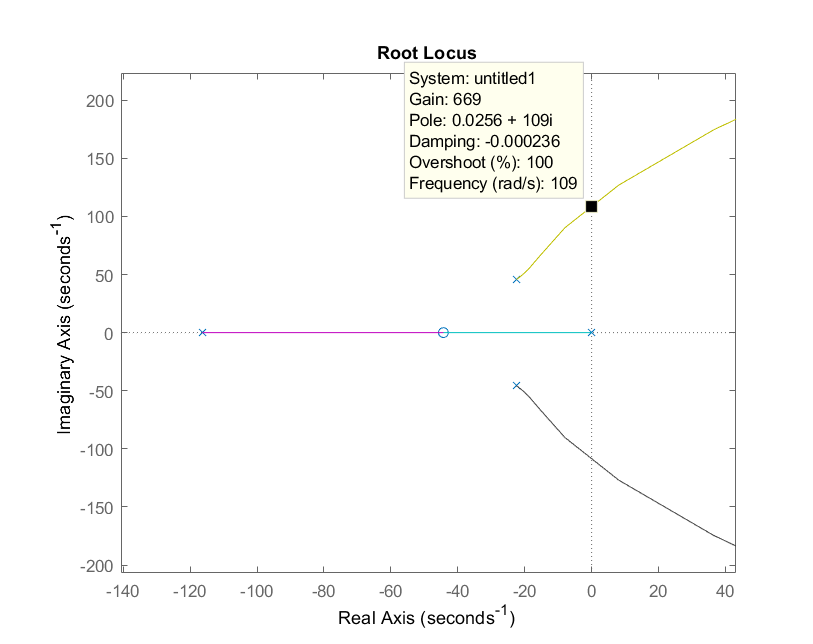
\includegraphics[scale=0.4]{rlocusconintegrador30kg.png}
	\caption{Lugar de raíces con el integrador.}
	\label{fig:lugar-de-raices-con-integrador-analog}
\end{figure}
\noindent \colorbox{yellow}{Cambiar la imagen de arriba por una que se vea mejor}

\noindent En la figura \ref{fig:lugar-de-raices-con-integrador-analog} se puede observar que, para que se mantenga la estabilidad del sistema, la ganancia del integrador ($K_{int\ }$) debe ser menor a 691. Teniendo esto en cuenta, en la figura \ref{fig:respuesta-al-escalon-con-k-1-M-30-analog} se muestra la respuesta al escal\'{o}n del sistema compensado con el integrador para una ganancia de $K_{int\ }=1$.  Es posible observar que, si bien no presenta oscilaciones, el tiempo de establecimiento es de aproximadamente 3 segundos. Por lo tanto, se decide aumentar el valor de ganancia hasta obtener una relaci\'{o}n aceptable entre el tiempo de respuesta y el sobrepico.

\begin{figure}[H]
	\centering
	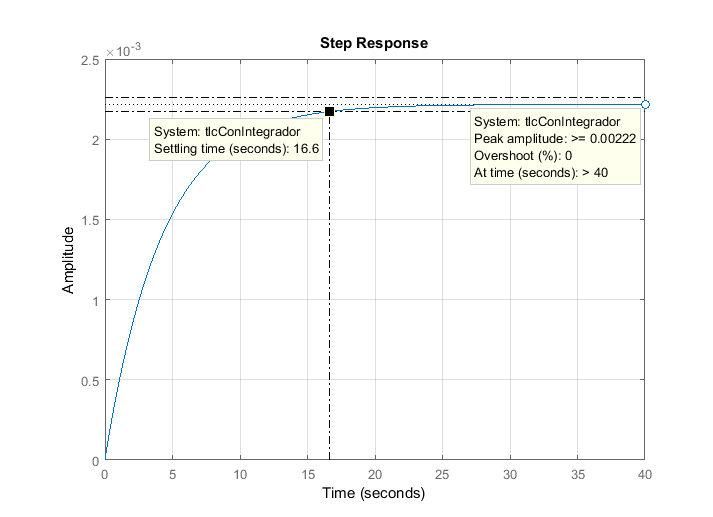
\includegraphics[scale=0.85]{stepresponseintegradorkint_1_m_30.png}
	\caption{Respuesta al escalón con integrador con $K_{int}$ =1 y M=30 Kg.}
	\label{fig:respuesta-al-escalon-con-k-1-M-30-analog}
\end{figure}

\noindent En la figura \ref{fig:respuesta-al-escalon-con-k-50-M-30}, se observa la respuesta al escal\'{o}n para una ganancia del integrador de $K_{int\ }=50$ que resulta en un tiempo de establecimiento de 0.6 segundos y un overshoot de 0\%. Por lo tanto, se adopta este valor de ganancia para el dise\~{n}o del integrador.

\begin{figure}[H]
	\centering
	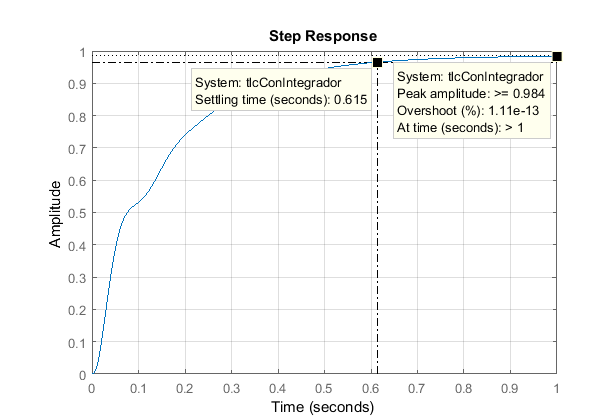
\includegraphics[scale=0.85]{stepresponseintegradorkint_50_m_30.png}
	\caption{Respuesta al escalón con integrador para $K_{int}$ =50 y M = 30 Kg.}
	\label{fig:respuesta-al-escalon-con-k-50-M-30}
\end{figure}

\noindent La respuesta al escal\'{o}n cuando la masa es de 1 Kg se muestra en la figura \ref{fig:respuesta-al-escalon-con-k-50-M-1}. All\'{i} se puede observar que el tiempo de crecimiento es de 0.74 s y el de establecimiento de 1.4 s. Adem\'{a}s, es posible notar que no presenta sobrepicos.

\begin{figure}[H]
	\centering
	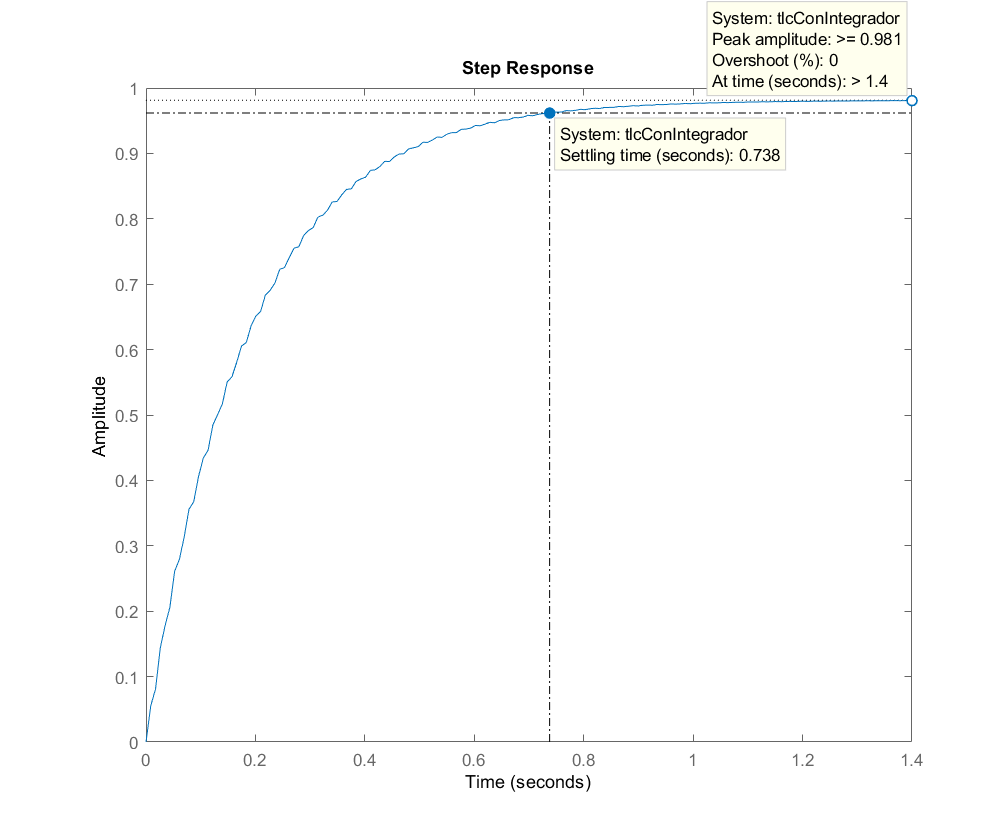
\includegraphics[scale=0.85]{stepresponseintegradorkint_50_m_1.png}
	\caption{Respuesta al escalón con integrador para $K_{int}$ =50 y M = 1 Kg.}
	\label{fig:respuesta-al-escalon-con-k-50-M-1}
\end{figure}



\subsection{Implementación circuital del integrador}

\noindent En la figura \ref{fig:circuito-integrador} se puede observar la topología y los valores utilizados en cada componente para el diseño del circuito integrador. 

\begin{figure}[H]
	\centering
	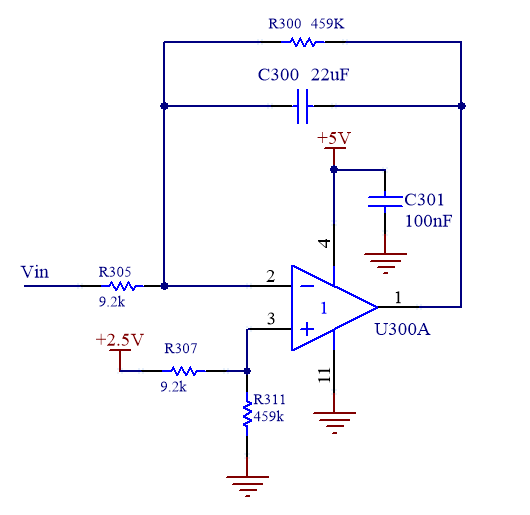
\includegraphics[scale=0.6]{Circuito-integrador.png}
	\caption{Implementación circuital del integrador.}
	\label{fig:circuito-integrador}
	\end{figure}
\section{Etapa de entrada}
\subsection{Cálculo de ganancia de entrada}

\noindent Tomando la TLC' que corresponde a la ganancia total de los bloques con el integrador ya incorporado, la ganancia resulta:

\begin{equation} 
	Ganancia_{TLC'} \simeq \frac{1}{H_{estim}} = - \frac{1}{260}
\end{equation}

\begin{figure}[H]
	\centering
	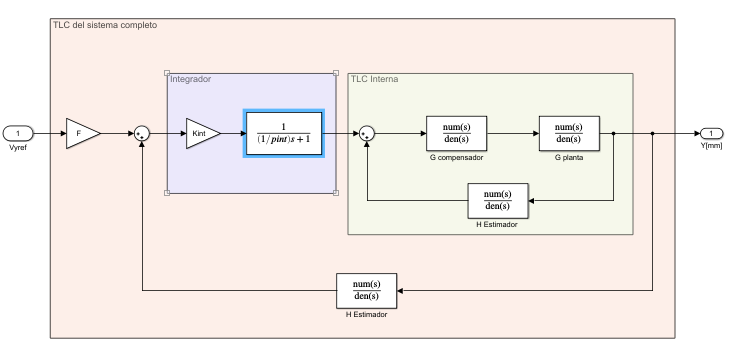
\includegraphics[scale=0.8]{Diagrama-en-bloques-compensador.png}
	\caption{Diagrama en bloques final.}
	\label{fig:diag-bloques-compensador}
\end{figure}

\noindent Por lo tanto teniendo tomando F=-1 y los rangos de posición de 1 mm a 5 mm como mínimo y máximo respectivamente se llega a lo siguiente:

\begin{equation} 
	Y[m] = F * (-\frac{1}{260})*V_{in} =\frac{1}{260}*V_{in} 
\end{equation}

\noindent La realimentación tiene un set-point de 3.4 V por lo tanto se le suma a Vin el mismo valor.

\noindent Los valores finales son:


\begin{table}[H]
	\begin{center}
		\begin{tabular}{| c | c |}
			\hline
			Y[mm] & $V_{in}[V]$\\ \hline
			5 & 4.7\\ \hline
			4 & 4.44 \\ \hline
			3 & 4.78\\ \hline
			2 &	3.92 \\ \hline		
		\end{tabular}
		\caption{Tensión de referencia $[V_{in}]$ Vs separación deseada [Y].}
		\label{tension-ref-vs-separacion-deseada}
	\end{center}
\end{table}

\subsection{Implementación circuital}

\noindent Para poder modificar la distancia de separación se ingresa al sistema con una tensión variable, la cual corresponde a una posición de referencia. Para ello se utiliza el circuito mostrado en la figura \ref{fig:etapa-de-entrada}.

\begin{figure}[H]
	\centering
	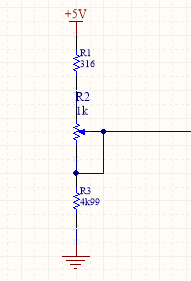
\includegraphics[scale=0.8]{Etapa-de-entrada.png}
	\caption{ Etapa de entrada.}
	\label{fig:etapa-de-entrada}
\end{figure}

 
 \noindent Se utiliza una resistencia variable de 1K y dos fijas. Para poder excursionar la tensión de referencia entre 3.92V y 4.7V, los valores de las resistencias R1 y R3 deben ser de 4911 y 313.5 respectivamente. 
 
\noindent Por lo tanto, adoptando un valor comercial para ellas, resulta:\\
\noindent R1 = 316 $\Omega$\\
\noindent R3 = 4990 $\Omega$
 
\noindent De esta forma, los valores de tensión para la referencia de posición quedan:\\
\noindent Tensión máxima= 4.69V\\
\noindent Tensión mínima = 3.96V
 
